\newcommand{\sigmaInel}{\sigma_\mathrm{inel}}
\newcommand{\sigmaAvg}{\sigma_\mathrm{avg}}

\newcommand{\qUmin}{qU_\mathrm{min}}

\newcommand{\Ekin}{E_\mathrm{kin}}
\newcommand{\nSource}{n_\mathrm{S}}
\newacronym{ft}{FT}{First Tritium}
\newacronym{knm1}{KNM1}{KATRIN Neutrino Mass Measurement 1}
\newacronym{mtd}{MTD}{measurement time distribution}
\chapter{Energy-Dependence of the Inelastic Scattering Cross Section}
\section{Introduction}
A $\upbeta$ electron's probability to scatter when travelling through the \gls{sts} depends on the scattering cross section $\sigma$ \eqref{eq:expectedScatteringCount}. The cross section $\sigma$ in turn depends on the kinetic energy $\Ekin$ of the electron: $\sigma \equiv \sigma(\Ekin)$. This dependence has been neglected in the modeling of the electron counts in section \ref{sec:scatProbs}. In a KATRIN measurement there exists a minimum retarding energy $\qUmin$ and only electrons with a kinetic energy greater than $\qUmin$ can reach the detector. A scattering cross section averaged over the kinetic energy of the electrons reaching the detector was assumed
\begin{equation}
    \sigma = \sigmaAvg = 
    \frac{1}{\Delta\Ekin} 
    \int_{\qUmin}^{\qUmin+\Delta\Ekin} \sigma(\Ekin) \d \Ekin 
    \quad \text{with} \quad
    \Delta\Ekin = \Eeff-\qUmin
    \fullstop
\end{equation}
Here, the ``effective endpoint'' $\Eeff$ denotes the highest kinetic energy of $\upbeta$ electrons reaching the detector. It does not necessarily match the endpoint of the tritium $\upbeta$ spectrum as experiment specific effects might shift it. $\Eeff=\SI{18575}{eV}$ is assumed. Instead of an average cross section an energy dependent formula can be used. Incorporating the energy dependence makes the model more complicated and slower to compute; neglecting it may lead to wrong results. More light will be shed on both aspects within this chapter.

\section{Cross Section Values}
\begin{figure}[t]
    \centering
    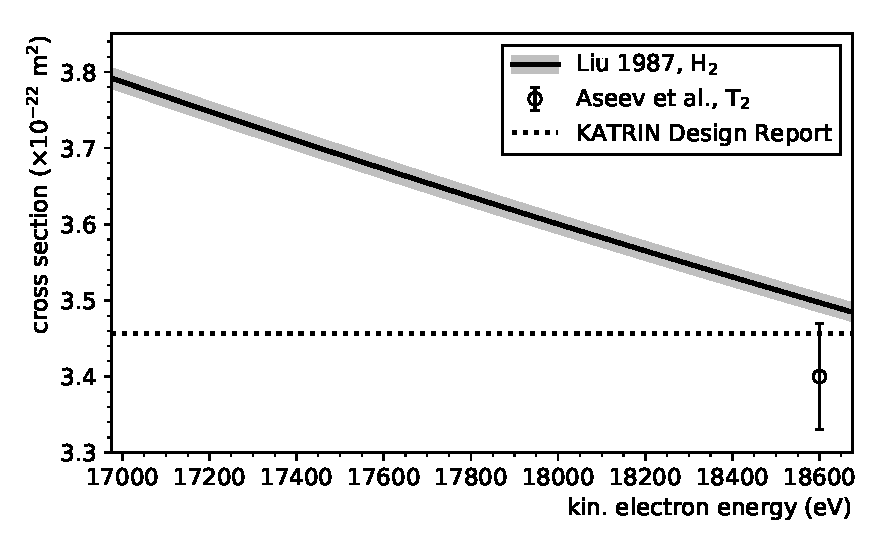
\includegraphics[width=\textwidth]{chapter/energyDependentCrossSec/fig/crossSecNoZoom.pdf}
    \xcaption{Inelastic cross section for non-relativistic electrons scattering from molecular hydrogen isotopologues}{Inelastic cross section for non-relativistic electrons scattering from molecular hydrogen isotopologues.}{Shown is the theoretical calculation by Liu along with its uncertainty \cite{Liu1973}, the measurement by Aseev et. al. at the Troitsk experiment \cite{Aseev2000} and the value stated in the KATRIN design report \cite{Angrik:2005ep}. (The values are also listed in table \ref{tab:crossSections}.) The depicted energy interval matches the measurement interval of the \glsentryfull{ft} campaign. {\color{red} FIX et al.}}
    \label{fig:scatCrossSec}
\end{figure}
The total scattering cross section is a sum of the cross section for elastic and inelastic scattering.
\begin{equation}
    \sigma(\Ekin) = \sigma_\mathrm{el} + \sigmaInel(\Ekin)
    \fullstop
\end{equation}
Only the energy dependence of the inelastic scattering cross section will be considered. This is justified for now as according to \cite{Angrik:2005ep} the cross section for elastic scattering is about an order of magnitude smaller than the one for inelastic scattering. An expression for the inelastic cross section for electrons scattering from hydrogen molecules can be found in \cite{Liu1973}. Two expressions are given, one for relativistic incident particles and one for non-relativistic incident particles. For the maximum relativistic $\beta$ factor of $\upbeta$ electrons from tritium decay one finds
\begin{equation}
\begin{split}
    \beta(\Ekin, m) &= 
    \sqrt{
        1-\frac{1}{
            (\frac{\Ekin}{m}+1)^2
        }
    } \\
    \beta_\mathrm{max} &= 
    \beta(\Eeff\approx\SI{18.6}{keV}, m_\elecIndex\approx\SI{511}{keV})\approx0.26
\end{split}
\end{equation}
Traveling at approximately a forth of the speed of light, the $\upbeta$ electrons are assumed to be non-relativistic. Then, the given expression for the energy dependent cross section is
\begin{equation}
	\label{eq:crossSecLiu}
    \sigma(\Ekin) =  
    (4 \pi a_0^2) \cdot
    \left(\frac{\Ekin}{R}\right)^{-1} \cdot
     \left[
        C_1 \cdot \ln{\left(\frac{\Ekin}{R}\right)} + C_2
    \right]
\end{equation}
with the Bohr radius $a_0$, the Rydberg energy $R$ and two constants given as
\begin{equation}
	\label{eq:crossSecLiuConstants}
    C_1 = 1.5487 
    \quad \text{and} \quad 
    C_2 = 2.2212\pm0.0434
    \fullstop
\end{equation}
Note that in other works $C_2=2.4036$ \cite{Liu1987} and $C_2=1.53$ \cite{Gerhart1975} are given. The value in \eqref{eq:crossSecLiuConstants} from \cite{Liu1973} was chosen to enable comparability with the KATRIN Design Report \cite{Angrik:2005ep}.

\begin{table}[t]
    \centering
    \xcaption{Energy-dependence of the inelastic scattering cross section}{Energy-dependence of the inelastic scattering cross section.}{Listed are important values with reference to KATRIN. Except for the measured value, they are obtained using \eqref{eq:crossSecLiu}. The values are given relative to an assumed endpoint of the measured spectrum $\Eeff=\SI{18575}{eV}$.}
    \begin{tabular}{lll}
        \toprule
         \makecell[tl]{kin. energy} & 
         \makecell[tl]{cross section \\ (\SI{e-22}{m})} & 
         \makecell[tl]{Note} \\
         \hline
         $\Eeff-\SI{1600}{eV}$ & 
         3.740 & 
         largest range in \gls{ft} campaign \\
         $\Eeff-\SI{90}{eV}$ & 
         3.469 & 
         largest range in \gls{knm1} campaign \\
         $\Eeff-\SI{30}{eV}$ & 
         3.459 & 
         KATRIN reference measurement interval \cite{Angrik:2005ep} \\
         $\Eeff-\SI{10}{eV}$ & 
         3.456 & 
         KATRIN reference value \cite{Angrik:2005ep} \\
         $\Eeff$ & 
         3.454 & 
         endpoint of tritium $\upbeta$ spectrum \\
         \SI{18600}{eV} & 
         $3.40\pm0.07$ & 
         measured at the Troitsk experiment \cite{Aseev2000} \\
         \bottomrule
    \end{tabular}
    \label{tab:crossSections}
\end{table}

Furthermore, the total inelastic scattering cross section was measured at the Troitsk experiment and the KATRIN Design Report states a reference value. The values are listed in table \ref{tab:crossSections}. The reference value matches the theoretical calculation using \eqref{eq:crossSecLiu} at a kinetic energy of $\Ekin\approx\SI{18564.4}{eV}$ which would be the center of a $\Delta\Ekin=\SI{20}{eV}$ KATRIN measurement interval. Note that in the KATRIN reference measurement interval $[\Eeff-\SI{30}{eV}, \Eeff]$ the cross section varies  $\sim\SI{0.14}{\percent}$. This variation is below its theoretical uncertainty given by \eqref{eq:crossSecLiuConstants}. In the measurement interval of the \gls{ft} campaign it varies $\sim\SI{8}{\percent}$.
    
\section{Motivation}
The motivation to implement an energy dependent cross section into the \gls{ssc} framework is two-fold:
\par{\textbf{Deep scans:} According to \cite{Groh2015} for a neutrino mass determination with the precision goals of KATRIN, the inelastic scattering cross section has to be known with an upper uncertainty of $\SI{0.0055e-22}{m}$ (\SI{0.16}{\percent}). This requirement might be surpassed by neglecting that the scattering cross section is not constant, but varies with energy. According to table \ref{tab:crossSections} the requirement is fulfilled in a measurement interval of $[\Eeff-\SI{30}{eV}, \Eeff]$. According to \eqref{eq:crossSecLiu} it is violated if the lower bound of the measurement interval is below \SI{18531}{eV}. Scans deeper into the tritium $\upbeta$ spectrum increase the count rates and hence, improve the statistic uncertainty on the neutrino mass. Also, for the search of sterile neutrinos deeper scans are necessary. On top of that, deeper scans have already been performed e.g. in the \gls{ft} campaign and help to establish an even better understanding of the KATRIN apparatus. In these cases the energy dependence is not negligible.}
\par{\textbf{Comparability:} A possible cross-check for software is its comparison to other software that was developed independently. \gls{ssc} is part of a data fitting suit. Other fitting software exists within the KATRIN collaboration that uses an energy dependent scattering cross section, e.g. FITRIUM \cite{Fitrium}. Furthermore, \gls{ssc} is commonly cross-checked against a Monte-Carlo particle tracking software called KASSIOPEIA \cite{KATRINCOL2019} which also implements an energy dependent scattering cross section.}
    
\section{Scattering Probabilities}
\subsection{Modelling}
\label{sec:energyDepScatProbsModel}
\begin{table}[ht]
    \centering
    \xcaption{Scattering probabilities}{The scattering probabilities}{averaged over all starting positions and starting angles in the \gls{wgts}. Both the values from a Monte Carlo (MC) simulation and the values according to \eqref{eq:averagedScatProbs} are given. The later ones can also be found in \cite{Groh2015, Kleesiek2014} and in the code of the \gls{ssc} framework \cite{KATRINCOL2019}.}
    \begin{tabular}{lll}
        \toprule
         \makecell[tl]{scattering count} & 
         \makecell[tl]{MC particle tracking \cite{Groh2015}} & 
         \makecell[tl]{equation \eqref{eq:averagedScatProbs}} \\
         \hline
         0 & $0.415 \pm 0.002$ & 0.41334 \\
         1 & $0.292 \pm 0.002$ & 0.29266 \\
         2 & $0.166 \pm 0.001$ & 0.16733 \\
         3 & $0.079 \pm 0.001$ & 0.07913 \\
         4 & $0.031 \pm 0.001$ & 0.03178 \\
         \bottomrule
    \end{tabular}
    \label{tab:scatProbs}
\end{table}
\begin{figure}[th]
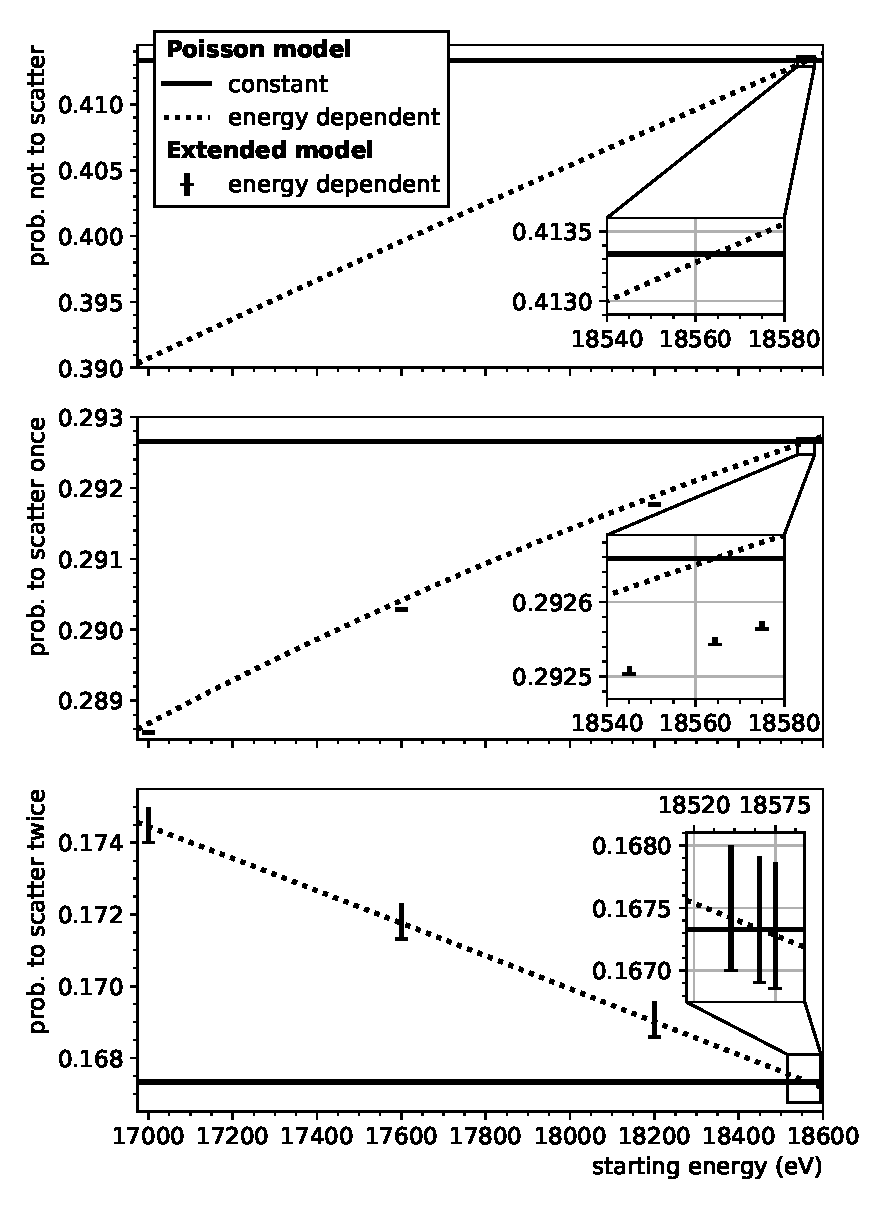
\includegraphics[width=\textwidth]{chapter/energyDependentCrossSec/fig/scatProbs123.pdf}
        \xcaption{Scattering probabilities}{Scattering probabilities.}{Shown are from top to bottom the probability for no, 1-fold and 2-fold scattering averaged over all starting positions and starting pitch angles of $\upbeta$ electrons. Depending on the required accuracy, for 1-fold and 2-fold scattering the Poisson model does not hold. The markers show an extended model as described in the text. Its numerical evaluation suffers from a one-sided uncertainty (of $\sim10^{-5}$ for 1-fold and $\sim10^{-3}$ for 2-fold scattering) depicted as uncertainty bars. The inset shows an energy span around the endpoint of the tritium $\upbeta$ spectrum. The full energy range matches the measurement interval of the \glsentryfull{ft} campaign.}
        \label{fig:energyDependentScatProbs}
\end{figure}
The energy-dependence of the scattering cross section enters into the calculation of the scattering probabilities \eqref{eq:scatProbs}. In the derivation the dependence on the starting energy $\Esource$ was neglected. Instead an average starting energy and hence, an average scattering cross section $\sigma(\SI{18564.4}{eV})=\SI{3.456e-22}{m^2}$ was assumed. For this case table \ref{tab:scatProbs} lists the scattering probabilities averaged over all starting positions and pitch angles in the \gls{wgts}.
In the energy dependent case the scattering cross section has to be adapted to the starting energy of the $\upbeta$ electrons. In other words, the scattering probabilities follow a Poisson distribution averaged over starting positions and pitch angles of $\upbeta$ electrons. Analogously to the derivation in section \ref{sec:scatProbs} they read:
\begin{subequations}
\label{eq:energydepScatProbsPoissonModel}
\begin{align}
    \mu(\Esource,\zSource,\thetaSource) =&
    \frac{\sigma(\Esource)}{\cos\thetaSource}
    \int_{\zSource}^{L/2} \rho(z)\d z \label{eq:energydepScatProbsPoissonExpectedScatCount} \\
    P_l(\Esource,\zSource,\thetaSource) =&
    \mathrm{Poisson}(\mu(\Esource,\zSource,\thetaSource),l) \label{eq:nonAveragedEnergydepScatProbsPoisson} \\
    \bar{P}_l(\Esource) =&
    \frac{1}{L \cdot (1-\cos(\thetaMax))} 
      \int_{-L/2}^{L/2}  
          \int_{0}^{\theta_{max}} 
            \sin(\thetaSource)
            \mathrm{Poisson}(\mu(\Esource,\zSource,\thetaSource),l)
          \d\thetaSource
      \d\zSource
      \label{eq:energydepScatProbsPoisson}
    \fullstop
\end{align}
\end{subequations}
Here, $\bar{P}_l(\Esource)$ in the final equation \eqref{eq:energydepScatProbsPoisson} denotes the probability of $l$-fold scattering for a $\upbeta$ electron with a starting energy $\Esource$ averaged over all starting positions and pitch angles. This model will be denoted Poisson model. It is expected to be accurate for the probability of no scattering $\bar{P}_0(\Esource)$.

But, depending on the required accuracy, for 1 or more scatterings this Poisson model does not necessarily hold. A scattering electron loses energy. Due to a lower energy the scattering cross section increases and the electron becomes more likely to scatter again. In other words, the probability of individual scattering processes are no longer independent. This violates one of the preconditions to model the scattering probabilities via a Poisson distribution. Another model is suggested. It assumes a constant gas density $\rho$, a fixed energy loss of $\epsilon$ per scattering and a source length of $L$:
\begin{subequations}
\label{eq:energydepScatProbsModel}
\begin{align}
    \mu(E,\thetaSource) =&
        \frac{\sigma(E)\rho L}{\cos\thetaSource} \\
    p_0(E,\thetaSource,n) =&
        \left(
            1-\frac{\mu(E,\thetaSource)}{N}
        \right)^n \\
    p_l(E,\thetaSource,n) =&
        \sum_{k=l}^{n}
        p_{l-1}(E,\thetaSource,k-1)
        \left(
            1-p_0(E-(l-1)\epsilon,\thetaSource,1)
        \right)
        p_0(E-l\epsilon,\thetaSource,n-k) \\
    \bar{p}_l(E,\thetaSource) =& 
        \frac{1}{L}
        \int_{0}^{L}
            p_l(E,\thetaSource,
                \left\lceil N \frac{\zSource}{L}\right\rceil
            )
        \d \zSource 
        \label{eq:energydepScatProbsZAverage} \\
      P^{\star}_l(\Esource,\thetaSource) =& 
        \lim_{N\rightarrow\infty} \bar{p}_l(\Esource,\thetaSource) 
        \label{eq:energydepScatProbsLimit} \\ 
    \bar{P}^{\star}_l(\Esource) =& 
    \frac{1}{1-\cos\thetaMax}
    \int_0^{\thetaMax}
        P^{\star}_l(\Esource,\thetaSource) 
        \d \thetaSource
        \label{eq:energydepScatProbs}
    \fullstop
\end{align}
\end{subequations}
Here, $\bar{P}^{\star}_l(\Esource)$ in the final equation \eqref{eq:energydepScatProbs} denotes the probability of $l$-fold scattering for a $\upbeta$ electron with a starting energy $\Esource$ averaged over all starting positions and pitch angles assuming a fixed energy loss $\epsilon$ per scattering. This model will be denoted extended model. A descriptive derivation is given in \mbox{appendix \ref{sec:energyDepOfScatProbsAppendix}}. 

The extended model is evaluated numerically as it includes one limit and two integrals. A balance between the numerical accuracy and the evaluation run time had to be found. Details can be found in the \mbox{appendix \ref{sec:energyDepOfScatProbsAppendixNumEval}}. The probability for 1-fold scattering could be calculated with an accuracy on the $10^{-5}$ level and for 2-fold scattering with an accuracy on the $10^{-3}$ level.

The suggested extended model is only valid for a fixed energy loss per scattering $\epsilon$. The value $\epsilon=\SI{14.1}{eV}$ was chosen as it is the most probable energy loss for electrons travelling through tritium gas according to \cite{Aseev2000}. A more accurate description would use the energy loss probability density. This has not yet been considered.

Figure \ref{fig:energyDependentScatProbs} shows the Poisson model along with the suggested extended model. The results are discussed in the following paragraphs.


\paragraph{Model compatibility}
 For 1-fold scattering the difference between the Poisson and the extended model is on the $10^{-4}$ level. For 2-fold scattering the accuracy of the numerical evaluation of the extended model is not yet sufficient to distinguish it from the Poisson model. Table \ref{tab:scatProbs} lists the scattering probabilities for an energy independent Poisson model and a reference cross section $\sigma(\SI{18564.4}{eV})=\SI{3.456e-22}{m}$ given in the KATRIN Design Report \cite{Angrik:2005ep}. It also lists the outcome of a Monte Carlo simulation taken from \cite{Groh2015}. As expected the energy dependent Poisson model recovers the energy independent model exactly at the corresponding energy of \SI{18564.4}{eV}. Furthermore, within the endpoint region of the tritium $\upbeta$ spectrum all models match the Monte Carlo simulation within its uncertainty.

\paragraph{Trend of energy-dependence}
For a decreasing starting energy of $\upbeta$ electrons the probability for no and 1-fold scattering also decreases while the probability for 2-fold scattering increases. This is expected for the following reasons. For a starting energy of $\Esource=\SI{18564.4}{eV}$ the expected amount of scatterings $\mu$ \eqref{eq:energydepScatProbsPoissonExpectedScatCount} averaged over all starting positions $\zSource$ and pitch angles $\thetaSource$ is
\begin{equation}
    \bar{\mu} = 
      \frac{1}{L \cdot (1-\cos(\thetaMax))} 
      \int_{-L/2}^{L/2}  
          \int_{0}^{\theta_{max}} 
            \sin(\thetaSource)
            \mu(\Esource,\zSource,\thetaSource)
          \d\thetaSource
      \d\zSource = 1.077
      \fullstop
\end{equation}
In other words, $\upbeta$ electrons with a starting energy near the endpoint of the tritium $\upbeta$ spectrum are expected to scatter around $\bar{\mu}=1.077$ times when travelling through the \gls{wgts}. If the starting energy decreases and hence, scattering becomes more likely it becomes more likely to scatter more than $\bar{\mu}$ times and less likely to scatter less than $\bar{\mu}$ times. Thus, the probability for no and 1-fold scattering decreases along with the starting energy of the $\upbeta$ electrons. At the same time the probability for more than 1 scatterings increases for lower starting energies. This intuitive reasoning is also reflected by deriving the scattering probabilities \eqref{eq:nonAveragedEnergydepScatProbsPoisson} for the starting energy where $\mu$ denotes the expected scattering count \eqref{eq:energydepScatProbsPoissonExpectedScatCount}
\begin{equation}
    \frac{\d P_l(\Esource,\zSource,\thetaSource)}
    {\d \Esource} =
    \underbrace{
        \mathrm{Poisson}(\mu(\Esource,\zSource,\thetaSource),l)
        \vphantom{\frac{\d \sigma(\Esource)}{\d \Esource}}
    }_{\geq 0} \cdot
    \underbrace{
        \left(
            \frac{l}{\mu(\Esource,\zSource,\thetaSource)} -1
        \right)
        \vphantom{\frac{\d \sigma(\Esource)}{\d \Esource}}
    }_{(*)} \cdot
    \underbrace{
    \frac{\int_{\zSource}^{L} \rho(z) \d z}
    {L \cos\thetaSource}
    \vphantom{\frac{\d \sigma(\Esource)}{\d \Esource}}
    }_{>0} \cdot
    \underbrace{
        \frac{\d \sigma(\Esource)}{\d \Esource}
    }_{<0} \fullstop
\end{equation}
 The sign of the derivative is determined by the sign of $(*)$ which follows approximately the above reasoning being negative for $l<\bar{\mu}$ and positive for $l>\bar{\mu}$.

\section{Performance and Accuracy Considerations}
\begin{figure}[th]
    \centering
    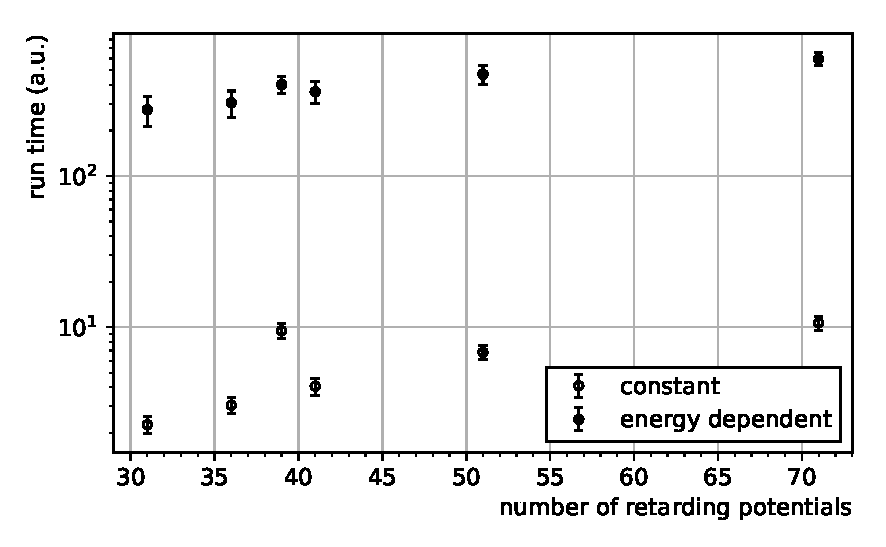
\includegraphics[width=\textwidth]{chapter/energyDependentCrossSec/fig/scatCrossSecRunTime.pdf}
    \xcaption{Run-time comparison between using an energy-dependent and -independent cross section}{Run-time comparison between using an energy-dependent and independent cross section.}{Shown are the run times for a fit of a simulated model to itself for different \gls{mtd}s. The \gls{mtd}s for the ranges 20, 25, 30, 40 and 50 \SI{}{eV} are taken from the KATRIN design report \cite{Angrik:2005ep} and have a rising number of retarding potentials. A further \SI{90}{eV}-wide \gls{mtd} of the \gls{knm1} campaign was used. It contains 39 retarding potentials. The corresponding run time lies above the trend line as the width of the measurement interval is wider.  For each \gls{mtd} 30 fits were performed. The run times were clocked for a constant and an energy-dependent cross section.}
    \label{fig:scatCrossSecRunTimes}
\end{figure}
The suggested extended model \eqref{eq:energydepScatProbsModel} at its current stage is computationally too expensive to be used in a fitting procedure. Note that a similar model has been derived for a fixed change of the pitch angle $\theta$ per scattering in \cite{Groh2015}. This model for angular changes is implemented in the \gls{ssc} software and can be used in fitting procedures. Though, an important difference is that the determination of the count rate requires an integral over the starting energy $\Esource$ in \eqref{eq:countsDependingOnPositionAndPitchAngle}. Hence, the energy dependent scattering probabilities have to be recomputed in every step of the numerical integration. This is not the case for the model considering the angular changes.

Albeit the energy dependent Poisson model might not fully hold in the case of an energy dependent cross section, figure \ref{fig:energyDependentScatProbs} shows that for larger measurement intervals it is more accurate than assuming energy independent scattering probabilities. Hence, it is a reasonable choice to implement the energy dependent Poisson model into the \gls{ssc} software. This was done. As mentioned the energy dependent scattering probabilities have to be recomputed in every step of the numerical integration in \eqref{eq:countsDependingOnPositionAndPitchAngle} over the $\upbeta$ electron energy. The impact on the run time was probed for 5 different \gls{mtd}s. They differ in the amount and range of retarding potentials. Both aspects should influence the run time. The run time should be approximately linear in the amount of retarding potentials. The run time should get longer the wider the range of the retarding potentials is as the numerically evaluated integral over energies in \eqref{eq:countsDependingOnPositionAndPitchAngle} then stretches over a wider range. Figure \ref{fig:scatCrossSecRunTimes} shows that the run times increase by a factor of approximately $40-120$ between assuming a constant cross section and an energy dependent one.

\section{Effect on Neutrino Mass Determination}
\begin{figure}[t]
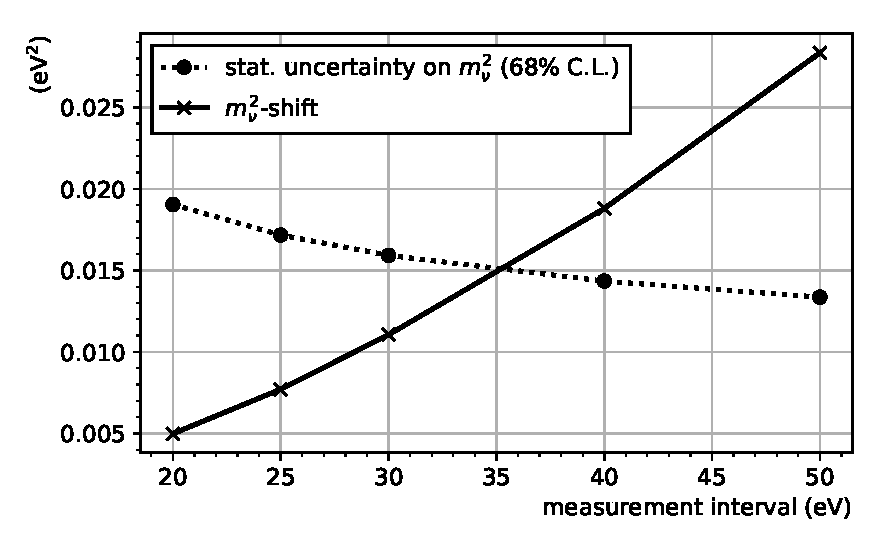
\includegraphics[width=\textwidth]{chapter/energyDependentCrossSec/fig/effectOnNuMass.pdf}
        \xcaption{Neutrino mass shift due to an energy dependent inelastic scattering cross section}{Neutrino mass shift due to an energy dependent inelastic scattering cross section}{as calculated by SSC for 5 measurement intervals. The configuration for the calculation, especially the \glsentryfull{mtd}, follows the KATRIN Design Report \cite{Angrik:2005ep}. For comparison the statistical uncertainty is plotted as well. It is derived from the profile likelihood. The lines between the 5 markers are linear interpolations.}
        \label{fig:energyDepCrossSecEffectOnNuMass}
\end{figure}
\todo{Numbers can not be reconciled with shifting the cross section. What to do about it?}
In order to determine the influence of the energy dependence of the scattering cross section on the neutrino mass determination the so-called ``shift method'' was used. A description can e.g. be found in \cite{SeitzM2019}. \todo{Write own description} In short, an integrated rate using the energy dependent Poisson model for the scattering probabilities was simulated and fitted to a model using the constant Poisson model. One obtains a deviation of the fitted and simulated neutrino mass, the neutrino mass shift. The procedure was repeated for multiple measurement intervals using the settings from the KATRIN Design Report \cite{Angrik:2005ep} for a 3-year measurement. A comparison of the statistical uncertainty on the neutrino mass and its shift is shown in figure \ref{fig:energyDepCrossSecEffectOnNuMass} depending on the measurement interval. For a measurement interval of approximately \SI{35}{eV} the shift and the statistical uncertainty are approximately equal
\begin{equation}
    \sigma(m_\nu) \approx 
    \sqrt{0.015}\SI{}{eV} = \SI{122}{meV} 
    \text{ (\SI{68}{\percent} C.L.)}
    \fullstop
\end{equation}

\paragraph{Extending the Measurement Interval}
In spring 2019 the so-called \gls{knm1} campaign started. The measurement interval was \SI{90}{eV}. The \gls{mtd} had been optimized according to the up-to-date status of the KATRIN experiment which did not match the KATRIN Design Report in all aspects. The study on the neutrino mass shift was redone scaling the \gls{mtd} of the \gls{knm1} campaign to 3 years and using the corresponding \gls{knm1}-settings. The neutrino mass shift then would be \SI{297}{meV}.


\section{Conclusion and Outlook}
The energy dependence of the scattering cross section enters into the calculation of the scattering probabilities. An accurate modelling of the energy dependent scattering probabilities is challenging due to performance reasons, but modelling them according to a Poisson distribution is possible. It was shown that the difference between the Poisson model and a more accurate model for 1-fold scattering is on the $10^{-4}$ level. The cases for more than 1 scatterings need further investigation. Also a fixed energy loss per scattering was assumed instead of a energy loss probability distribution. Future work might consider these aspects and what influence a more accurate modeling on the scattering probabilities has on the neutrino mass determination.

Given the KATRIN uncertainty budget, when modeling the energy dependent scattering probabilities via a Poisson distribution, the energy dependence of the scattering cross section is not negligible for measurement intervals that extend more than \SI{35}{eV} below the endpoint of the tritium $\upbeta$ spectrum.

Including the energy dependence in the analysis increases the run time of the fitting procedure significantly. Future work might consider to precalculate the scattering probabilities for different fixed energies and use interpolation techniques for energies in-between the fixed ones.